\documentclass[a4paper,12pt]{article}
\usepackage[utf8]{inputenc}
\usepackage[german]{babel}
\usepackage{amsmath}
\usepackage{amssymb}
\usepackage{amsthm}
\usepackage{geometry}
\usepackage{graphicx}
\usepackage[hidelinks]{hyperref}

\geometry{margin=2.5cm}

\theoremstyle{definition}
\newtheorem{definition}{Definition}
\newtheorem{beispiel}{Beispiel}
\newtheorem{satz}{Satz}

\title{Zufall in der Mathematik}
\author{Stephan Epp}
\date{\today}

\begin{document}
	
\maketitle

\tableofcontents
\newpage

\section{Einführung}

Zufall wird in der Mathematik beschrieben für diskrete und kontinuierliche Ereignisse. Diskrete Ereignisse sind dabei die natürlichen Ereignisse, die sich jeder gut vorstellen kann. Ein diskretes Ereignis ist zum Beispiel das Würfeln eines Würfels. Ein Würfel hat sechs Seiten. Dabei hat jeden Seite des Würfels eine Augenzahl, dass jede Augenzahl von $1, \ldots, 6$ auf jeweils einer Würfelseite abgebildet ist. Es stellt sich die Frage, wenn jemand den Würfel einmal würfelt, auf welche Augenzahl der Würfel fällt? Da es sechs Seiten gibt, kann es sein, dass der Würfel bei einem Wurf zufällig auf die Augenzahl $3$ fällt. Ist die $3$ auf dem Würfel deshalb bevorzugt, weil der Würfel beim Wurf auf die Augenzahl $3$ gefallen ist? Kommt es zufällig öfter vor, dass der Würfel auf die Augenzahl $3$ fällt? Nein, der Würfel hat sechs gleich große Seiten und keine der Seiten des Würfels ist durch die Art des Würfels bevorzugt.

\section{Grundlagen}

Um jede Unruhe über den Ausgang des Zufalls allen Beteiligten zu nehmen, wird der Zufall für diskrete Ereignisse mit Hilfe der Mathematik beschrieben und analysiert. 

\subsection{Definition}

Für das diskrete Ereignis, bei dem ein Würfel einmal geworfen wird, können folgende diskrete Ereignisse zufällig eintreten. Der Würfel kann auf die Augenzahl $1$ fallen, der Würfel kann auf die Augenzahl $2$ fallen, ..., der Würfel kann auf die Augenzahl $6$ fallen. Dabei ist jeder Fall des Würfels auf eine andere Augenzahl ein Ereignis. Es gibt damit also sechs Ereignisse beim Würfeln des Würfels mit sechs Seiten.  

Ein \textit{Versuch} beschreibt das Vorhaben zum Beispiel einen Würfel zu würfeln. In diesem Versuch können unterschiedliche Ereignisse zufällig eintreten. \textit{Die Menge aller Ereignisse für einen Versuch}, die zufällig eintreten können, wird definiert mit $\Omega$. Um nun zu sagen, wie zufällig es ist, dass der Würfel beim Wurf auf die Augenzahl $3$ fällt, muss nur dieses Ereignis ins Verhältnis zu allen möglichen Ereignissen gesetzt werden. Damit ergibt sich als Wert für den Zufall des Ereignisses, dass der Würfel beim Wurf auf die Augenzahl $3$ fällt, die \textit{Wahrscheinlichkeit} von $\frac{1}{6}$. Es fällt auf, dass für jedes Ereignis dieses Versuches gilt, dass der Würfel beim Wurf auf die Augenzahl $k$ fällt, die \textit{Wahrscheinlichkeit} $\frac{1}{6}$ hat, $k \in \Omega = \{1, \ldots, 6\}$. Denn der Würfel hat ja sechs gleich große Seiten und keine der Seiten des Würfels ist durch die Art des Würfels bevorzugt. Ist die Summe aller Wahrscheinlichkeiten der Zufälle aller Ereignisse insgesamt $1$, wurden alle Ereignisse des Versuchs berücksichtigt und der Versuch ist \textit{mathematisch vollständig beschrieben}.

Für Versuche, die durch diskrete Ereignisse beschrieben werden, ist die Überprüfung der vollständigen mathematischen Beschreibung notwendig. Erst dann liegt eine mathematische Beschreibung vor, auf deren Grundlage weitere Ereignisse für diesen Versuch betrachtet und analysiert werden können. Für den Versuch einen Würfel einmal zu würfeln kann man sich auch fragen, wie wahrscheinlich der Zufall für das Ereignis ist, dass der Würfel nicht auf den Augenzahl $3$ fällt. Das ist komplizierter, im Allgemeinen. Glücklicherweise aber betrachten wir diskrete Ereignisse. Deshalb lässt sich die Wahrscheinlichkeit für den Zufall des Ereignisses, dass der Würfel nicht auf die Augenzahl $3$ fällt, wie folgt \textit{abzählen}. Die Wahrscheinlichkeit für den Zufall des Ereignisses, dass der Würfel nicht auf die Augenzahl $3$ fällt, ist dieselbe für den Zufall der Ereignisse, dass der Würfel auf die Augenzahl $1, 2, 4, 5$ oder $6$ fällt. Dies sind fünf Ereignisse. Damit ergibt sich eine Wahrscheinlichkeit für den Zufall des Ereignisses, dass der Würfel nicht auf die Augenzahl $3$ fällt, von $\frac{5}{6}$.

\subsection{Zufallsvariable}

Für Versuche, die durch diskrete Ereignisse beschrieben werden, ist es für die Analyse manchmal hilfreich, eine Zufallsvariable zu verwenden. Dabei beschreibt die Zufallsvariable den Zufall für das Ereignis variabel für den konkreten Ausgang. Zum Beispiel kann für den Versuch, einen Würfel zu würfeln, eine Zufallsvariable definiert werden durch 
\begin{align}
	\label{math:var-x}
	X = \{\text{Anzahl der Augen, auf die der Würfel fällt}\}.
\end{align}

Es fiel auf, dass für jedes Ereignis dieses Versuches gilt, dass der Würfel beim Wurf auf die Augenzahl $k$ fällt, die \textit{Wahrscheinlichkeit} $\frac{1}{6}$ hat, $k \in \{1, \ldots, 6\}$. Mit der Zufallsvariable ist diese Beobachtung nun so beschreibbar $P(X = k) = \frac{1}{6}$, wobei $P$ für Probability steht.

\subsection{Erwartungswert}

Bei dem Versuch, den Würfel zu würfeln, ist es vor dem Versuch von Bedeutung, zu ermitteln, welcher Ausgang des Versuches zu erwarten ist. Für Versuche, die durch diskrete Ereignisse beschrieben werden, wird der Erwartungswert $E$ für eine Zufallsvariable $X$ so berechnet:
\begin{align}
	E[X] &= \sum_{k \in \Omega} k \cdot P(X = k).
\end{align}
Für die Zufallsvariable $X$ von (\ref{math:var-x}) ergibt sich damit ein Erwartungswert von
\begin{align}
	E[X] &= \sum_{k \in \{1, \ldots, 6\}} k \cdot P(X = k) \\
		 &= 1 \cdot P(X = 1) + \ldots + 6 \cdot P(X = 6) \\
		 &= 1 \cdot \frac{1}{6} + \ldots + 6 \cdot \frac{1}{6} \\
		 &= 3,5.
\end{align}
Das bedeutet, bevor wir den Würfel einmal gewürfelt haben, erwarten wir, dass der Würfel auf die Augenzahl 3,5 fällt. Diese Augenzahl gibt es nicht. Der Erwartungswert aber beschreibt formal am genauesten, welcher Ausgang bei diesem Versuch wirklich zu erwarten ist. Denn erst wenn wir diesen Versuch oft wiederholen, ist es interessant, wie der tatsächliche Ausgang des Versuches vom Erwartungswert abweicht.

\section{3-SAT}

Gegeben sei eine 3-KNF Formel $\psi$ mit $m$ Klauseln $C_1, \dots, C_m$ und $n$ Variablen $x_1, \dots, x_n$. Die Variablen $x_i$ können nur einen Wert aus $\{0, 1\}$ annehmen. Jede Klausel $C_j$ enthält genau 3 Literale. Ein einfacher Algorithmus, der Zufall gebraucht, ermöglicht es, eine Approximationsgüte von $7/8$ zu erreichen. Das heißt, dass im Erwartungswert mindestens $87.5\%$ aller erfüllbaren Klauseln von $\psi$ erfüllt werden. Warum werden mit diesem Algorithmus $87.5\%$ aller erfüllbaren Klauseln erfüllt und warum ist das gut? Um $100.0\%$ aller erfüllbaren Klauseln von $\psi$ zu erfüllen, ist eine exponentielle Laufzeit in der Anzahl $n$ der Variablen nötig, die alle Zuweisungen von $\{0, 1\}$ zu den Variablen $x_i$ prüft. Daher verwendet man in der Praxis auch gute Lösungen, die nicht optimal sind, aber dafür effizient berechnet werden können.

Die Arbeitsweise des Algorithmus mit Zufall für 3-KNF ist:
\begin{enumerate}
	\item Für jede Variable $x_i$:
	\begin{itemize}
		\item[-] Setze $x_i = 1$ (Wahr) mit Wahrscheinlichkeit $\frac{1}{2}$, d.h., $P(x_i=1) = \frac{1}{2}$
		\item[-] Setze $x_i = 0$ (Falsch) mit Wahrscheinlichkeit $\frac{1}{2}$, d.h., $P(x_i=0) = \frac{1}{2}$
	\end{itemize}
	\item Die Zuweisungen der Werte $\{0, 1\}$ zu den Variablen $x_i$ erfolgen unabhängig voneinander.
\end{enumerate}
\textbf{Wahrscheinlichkeit für eine Klausel}: Eine Klausel $C_j = (l_1 \lor l_2 \lor l_3)$ ist nur dann nicht erfüllbar bzw. Falsch, wenn alle drei Literale in ihrer Interpretation jeweils den Wert Falsch haben. Da den Variablen unabhängig voneinander und mit Wahrscheinlichkeit $1/2$ ein Wert aus $\{0, 1\}$ zugewiesen wird, gilt:
\begin{equation}
	P(C_j \text{ ist Falsch}) = \left(\frac{1}{2}\right)^3 = \frac{1}{8}
\end{equation}
Die Wahrscheinlichkeit, dass die Klausel $C_j$ erfüllt ist, beträgt somit:
\begin{equation}
	P(C_j \text{ ist Wahr}) = 1 - P(C_j \text{ ist falsch}) = 1 - \frac{1}{8} = \frac{7}{8}
\end{equation}
\textbf{Erwartungswert der erfüllten Klauseln}: Wir definieren Indikatorvariablen $Y_j$ für $j = 1, \dots, m$:
\begin{equation}
	Y_j = 
	\begin{cases} 
		1, & \text{falls } C_j \text{ erfüllt ist} \\
		0, & \text{sonst}
	\end{cases}
\end{equation} 
Die Gesamtzahl der erfüllten Klauseln ist die Zufallsvariable $Y = \sum_{j=1}^{m} Y_j$. Aufgrund der Linearität des Erwartungswerts gilt:
\begin{align}
	E[Y] &= E\left[\sum_{j=1}^{m} Y_j\right] \\
	&= \sum_{j=1}^{m} E[Y_j] \\
	&= \sum_{j=1}^{m} P(Y_j = 1) \\
	&= \sum_{j=1}^{m} \frac{7}{8}.
\end{align}
Die erwartete Gesamtzahl aller erfüllten Klauseln beträgt damit also $\frac{7}{8}m$. Sei $O$ die optimale Anzahl an Klauseln, die in $\psi$ erfüllt werden können. Dann kann $O$ höchstens alle $m$ Klauseln erfüllen, also $O \le m$. Damit ergibt sich
\begin{equation}
	E[Y] = \frac{7}{8}m \ge \frac{7}{8} O.
\end{equation}
Das bedeutet, die Lösung des Algorithmus mit Zufall für 3-KNF erfüllt im Erwartungswert mindestens $\frac{7}{8}$ aller Klauseln der optimalen Anzahl an Klauseln, die überhaupt in $\psi$ erfüllt werden können. Die Laufzeit dieses Algorithmus mit Zufall für 3-KNF ist linear in der Anzahl der Klauseln und Variablen.

\subsection{Implementierung}

Der Algorithmus mit Zufall für 3-KNF wurde in Python implementiert. Es wurden Experimente durchgeführt. Abbildung \ref{fig:experiments} zeigt die Ergebnisse der Experimente.
\begin{figure}[htbp]
	\centering
	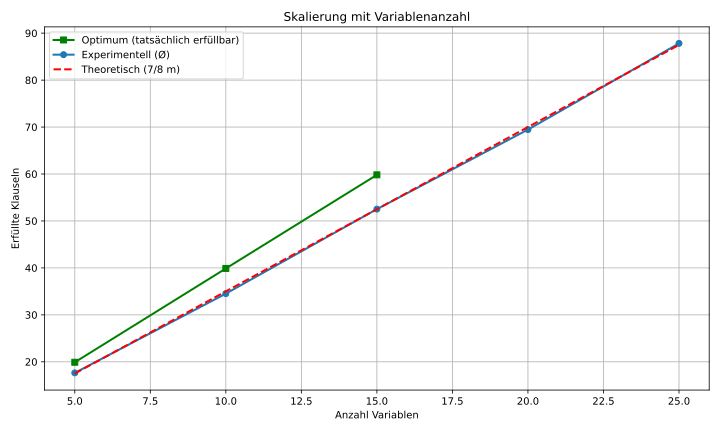
\includegraphics[width=0.8\textwidth]{../experiment-results.pdf}
	\caption{Experimentelle Ergebnisse des 3-SAT Algorithmus}
	\label{fig:experiments}
\end{figure}
Auf der x-Achse ist die Anzahl der Variablen und auf der y-Achse die Anzahl erfüllter Klauseln aufgetragen. In grün eingezeichnet ist die Anzahl der erfüllbaren Klauseln. In blau eingezeichnet ist die Anzahl der erfüllten Klauseln durch den 3-KNF Algorithmus mit Zufall und in rot eingezeichnet ist die erwartete Anzahl erfüllter Klauseln durch den 3-KNF Algorithmus mit Zufall.

Beobachtbar ist, dass die Anzahl der erfüllten Klauseln durch den 3-KNF Algorithmus mit Zufall der theoretischen erwarteten Anzahl erfüllter Klauseln entspricht. Bis zu einer Anzahl von 15 Variablen ist die Anzahl der erfüllten Klauseln durch den 3-KNF Algorithmus mit Zufall nicht so hoch wie die optimale, d.h. maximale, Anzahl erfüllbarer Klauseln.

\section{Zusammenfassung}
\subsection{Ausblick}
	
\end{document}